\chapter{Planification du projet  \guy{Raph}}

Le projet est divisé en cinq phases: l'analyse, la planification, la conception, la construction et le déploiement (voir le diagramme de Gantt en figure \ref{gantt_1}).

La phase d'analyse débute par la prise en main de E-YAKA afin d'ensuite pouvoir définir le sujet dans son ensemble, puis de définir les technologies qui seront utilisées. Il s'agit dans un premier temps, d'une phase d'échange avec les encadrants du projet pour préciser les travaux à réaliser au cours de l'année et pour rédiger le cahier des charges.

La phase de planification qui dure tout au long du premier semestre, est une phase essentielle pour le bon déroulement du projet car elle permet d’établir la feuille de route du projet. Elle spécifie et répartit les tâches ainsi que les responsabilités au sein du groupe. Elle permet de regrouper la synchronisation des tâches, les indicateurs de délais et les contraintes organisationnelles en s'appuyant sur l’outil de planification MS Project. Par exemple, des temps de travail partagés, d'échange entre les membres du groupe et d'évaluation de l'avancement du projet ont régulièrement lieu les jeudis après-midi.

La phase de conception s'oriente autour de la précision et de la définition complète du cahier des charges. Elle permet de préparer la phase de construction qui vient juste après.

La phase de construction consiste à implanter les systèmes de traçage, à intégrer la mise en forme des résultats et à étudier les résultats obtenus.

La phase de déploiement consiste à livrer le projet et les résultats obtenus sous diverses formes. Deux démonstrations du projet seront effectuée avec les encadrants et le rapporteur. Lors d’un showroom, ce projet sera présenté aux étudiants, aux enseignants et aux industriels. Les rapports ainsi que le code implémenté sera de même livré aux encadrants.


  \begin{figure}
    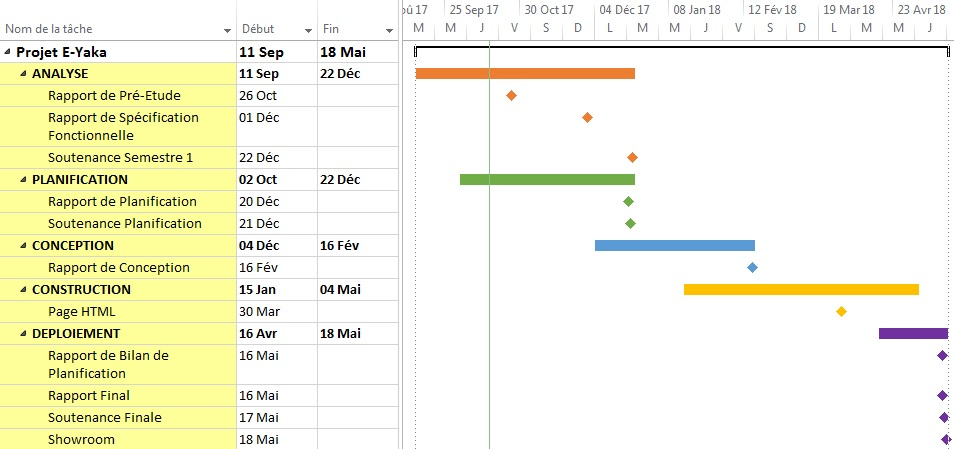
\includegraphics[width=1\textwidth]{images/gantt1.jpg}
    \caption{Diagramme de Gantt 1}
    \label{gantt_1}
  \end{figure}
